\chapter{Sparse naive Bayes}\label{ch:snb}

Naive Bayes was first introduced in the early 60s by~\cite{original_naive_bayes} for text documents classification.
It is a simple model assuming the independence of the features, given the label.
Despite this naive presupposition,
naive Bayes remains an engaging model for large scale datasets because of its low complexity.
The time complexity to train a model is asymptotically $\cO\left( n \cdot p \right)$,
where $n$ and $p$ are the number of samples and the number of features respectively.
Another appealing propriety is that naive Bayes can be trained in an online fashion,
as new data points come in a sequential order.
It can be particularly helpful if the dataset doesn't fit in memory.
Furthermore, distributed implementations could even be considered in order to speed up the learning process.

In this chapter, classical naive Bayes along with a few notations are briefly introduced.
Then, a sparse version of naive Bayes is presented,
allowing in particular to perform feature selection.

\section{Reminders on vanilla naive Bayes}\label{sec:naive_bayes}

In this section, we recall briefly the naive Bayes model in the specific case of binary classification,
and some details regarding the training phase under the bernoulli, multinomial and gaussian underlying assumptions.
Most key results can naturally be extended to the multiple classes setting.

Let $n$ and $p$ be two integers, $X \in \R^{n \times p}$ a design matrix
and $\yy \in \bset^n$ the associated target vector.
The negative and the positive classes are noted $\cC_-$ and $\cC_+$ respectively,
and will be indifferently substituted with their respective labels.

\subsection{General settings}\label{subsec:nb_general}

Note $\left( \cX,\, \cY \right)$ the pair of random variables that generated the samples and targets $X$ and $\yy$.
The goal is to explain $\yy$ given $X$, that is, finding the posterior probabilities $\Pr(\cC_\pm \mid \cX)$.
Given these probabilities, a new observation $\xx \in \R^p$ is classified according to the highest
posterior probability between the two classes
\begin{equation}\label{eq:nb_inference}
    y\left( \xx \right) = \underset{\cC \in \bclasses}{\argmax} \Pr\left( \cC \mid \xx \right)
\end{equation}
To do so, we combine the use of Bayes rule and make the (very) naive assumption that
all the features are independent given the class, that is
\begin{equation}
    \Pr\left( \cX = \xx \mid \cC_\pm \right) = \prod_{j = 1}^p \Pr(\cX_j = x_j \mid \cC_\pm)
    ,\qquad
    \Pr(\cC_\pm \mid \cX = \xx) = \frac{\Pr(\cX = \xx \mid \cC_\pm) \cdot \Pr(\cC_\pm)}{\Pr(\cX = \xx)}
\end{equation}
On the right hand side,
the denominator $\Pr(\cX = \xx)$ does not depend on the class $\cC_\pm$.
It is therefore not required to evaluate it in order to perform the inference described in~\ref{eq:nb_inference}.
Thus, we only need to estimate the probabilities $\Pr(\cC_\pm)$ and $\Pr(\xx \mid \cC_\pm)$.
The former are simply data averages, i.e.\ the frequencies of the positive and negative classes in the observed data.
As for the latter probabilities $\Pr\left( \xx \mid \cC_\pm \right) = \prod_{j = 1}^p \Pr(x_j \mid \cC_\pm)$,
they can be modeled by a plethora of distribution families, depending on the prior knowledge we have on the data.
The distribution is typically parametrized by some vector $\btheta \in \R^m$.
The probabilities are usually computed by maximizing the likelihood $\cL$,
or equivalently the log-likelihood $\lglh = \log\cL$, of the observed data.
\begin{equation*}
    \lglh\left( \btheta \right) = \sum_{i = 1}^n \Pr\left( \xx_i \mid y_i \,; \btheta \right)
\end{equation*}
We present now 3 meaningful cases, where the prior distributions of $\Pr(\xx \mid \cC_\pm)$ are either
gaussian, bernoulli or multinomial.
Let $\cI_\pm = \left\{ i \in \pset \mid y_i = \cC_\pm \right\}$ be the sets containing the
indexes of the positive and negative data points.
We also note for each class $\cC_\pm$ their cardinalities and empirical sums respectively, as follows:
\begin{equation*}
    n^\pm = | \cI_\pm |,
    \qquad\qquad
    \ff^\pm = \sum_{i \in \cI_\pm} \xx_i
\end{equation*}

\subsection{Gaussian naive Bayes}\label{subsec:gnb}

In this case the observed data conditioned on its label is modeled by the gaussian distribution
$\cN( \bmu^\pm, \Sigma^\pm )$.
It is the most common configuration because it can account for continuous data and the normal distribution constitures
a decent prior in many cases by virtue of its high entropy.
Note that the covariances $\Sigma^\pm \in \R^{p \times p}$
are diagonal as a result of the independence assumption that we made.
\begin{equation*}
    \Pr\left( \xx \mid C_\pm \right) =
    \frac{1}{\sqrt{(2\pi)^p\det(\Sigma_\pm)}}
    \exp\left( -\frac{1}{2}(\xx - \bmu_\pm)^\top\Sigma^{-1}(\xx - \bmu_\pm) \right)
\end{equation*}
By denoting $\sigma_j = \Sigma_{j j}$, the log-likelihood can be written
\begin{equation*}
    \begin{split}
        \lglh_g\left( \bmu_+,\, \ssigma_+,\; \bmu_-,\, \ssigma_-\right ) &=
            \sum_{j = 1}^p \Bigg[
                \sum_{i \in \cI_+}
                    -\frac{1}{2} \log \left( 2\pi \right)
                    -\log \sigma_j^+
                    -\frac{(x_j - \mu^+_j)^2}{2{\sigma^+_j}^2}\\
                &\qquad\quad+ \sum_{i \in \cI_-}
                    -\frac{1}{2} \log \left( 2\pi \right)
                    -\log \sigma_j^-
                    -\frac{(x_j - \mu^-_j)^2}{2{\sigma^-_j}^2}
            \Bigg]
    \end{split}
\end{equation*}
Even if $\lglh_g$ is not concave, it maximizer admits a closed-form solution
(readily shown to be the point where the gradient is null)
\begin{align*}
    \bmu^\pm = \frac{\ff^\pm}{n^\pm}
    ,\qquad\quad
    \ssigma^\pm = \sqrt{\frac{1}{n^\pm} \sum_{i \in \cI^\pm} (\xx_i - \bmu^\pm)^2}
\end{align*}

\subsection{Bernoulli naive Bayes}\label{subsec:bnb}

The Bernoulli distribution assumes that the design matrix is binary,
that is $X \in \zoset^{n \times p}$.
Even though this situation isn't very prevalent in practice, it has a simple and elegant solution.
In order to model the conditional probabilities, we may assume the existence of
$\btheta^+,\, \btheta^- \in \left( 0, 1 \right)^p$
such that for any data point $\xx \in \R^p$,
\begin{equation*}
    \Pr\left( x_j \mid \cC_\pm \right) = (\theta^\pm_j)^{x_j} \cdot (1 - \theta^\pm_j)^{1 - x_j}
\end{equation*}
It yields that $\log \Pr\left( \xx \mid \cC_\pm \right) =
\xx^\top\log\btheta^\pm + (\1 - \xx)^\top\log\left( \1 - \btheta^\pm \right)$
and finally
\begin{align}\label{eq:bernoulli_snb_ll}
    \lglh_b\left( \btheta^+,\, \btheta^- \right)
    &= \sum_{i \in \cI^+} \log \Pr\left( \xx_i \mid \cC_+ \right)
        + \sum_{i \in \cI^-} \log \Pr\left( \xx_i \mid \cC_- \right)\nonumber\\
    \begin{split}
        &= \ff_+^\top\log\btheta^+ + (n_+\1 - \ff_+)^\top\log\left( \1 - \btheta^+ \right)\\
        &\qquad+ \ff_-^\top\log\btheta^- + (n_-\1 - \ff_-)^\top\log\left( \1 - \btheta^- \right)
    \end{split}
\end{align}
The independence assumption makes the optimization problem decomposable across features;
it reduces to $p$ simpler maximizations, each of them being concave and admitting a closed-form solution.
Finally, we find that
\begin{equation*}
    \theta_\pm^\star = \frac{f^\pm}{n^\pm}
    ,\qquad\qquad
    \text{which are simply the averages of each class.}
\end{equation*}

\subsection{Multinomial naive Bayes}\label{subsec:mnb}

Multinomial naive Bayes generalizes the Bernoulli version
as it supposes that $X \in \N^{n \times p}$ is generated by the following underlying distribution
\begin{equation}\label{eq:multinomial_pr}
    \Pr\left( \xx \mid \cC_\pm \right) =
        \frac{\big( \sum_{j = 1}^p x_j \big)!}
            {\prod_{j = 1}^p x_j!} \cdot \prod_{j = 1}^p (\theta^\pm_j)^{x_j}
\end{equation}
In the special case where $X \in \zoset^{n \times p}$ we recover the above Bernoulli formulation.
It is parametrized by $\btheta^+,\, \btheta^- \in \left( 0,\, 1 \right)^p$, and they must satisfy
$\1^\top\btheta^+ = \1^\top\btheta^- = 1$ for~\ref{eq:multinomial_pr} to be a proper distribution.
Note that this model is still valid in the more general case
where we only assume the data to be non-negative, $X \in \R_+^{n \times p}$.
Hence, it is not as restrictive as it may appear at first sight,
as it is applicable to a large number of datasets.
The log probability is given by
\begin{equation*}
    \log\Pr\left(\xx \mid \cC_\pm\right) =
        \xx^\top\log\btheta_\pm + \log\frac{\big(\sum_{j = 1}^p x_j\big)!}{\prod_{j = 1}^p x_j!}
\end{equation*}
and the log-likelihood reduces to (after removing the constant terms)
\begin{equation}\label{eq:multinomial_snb_ll}
    \lglh_m\left(\btheta^+,\, \btheta^-\right) = \ff_+^\top\log\btheta^+ + \ff_-^\top\log\btheta^-
\end{equation}
which is again decomposable across features.
It turns out that the optimums are
\begin{equation*}
    \btheta_\pm^\star = \frac{\ff^\pm}{\1^\top\ff^\pm}
\end{equation*}
\bigbreak
In the models presented above, the time complexity to train the naive Bayes classifier is $\cO(n \cdot p)$.
With a larger number of classes besides $\cC^-$ and $\cC^+$, say $k$ classes, this complexity is multiplied by $k$.
On top of this low asymptotic complexity,
the solutions can be computed in closed-form, which makes the effective computation cost very low.
In comparison, no closed-form solution exist for the Lasso, for logistic regression~\cite{logistic_regression},
and for SVMs~\cite{svm}.
These models are usually trained by employing more costly gradient-descent based algorithms to find the global optimum.

\subsection{Decision boundary}\label{subsec:nb_bound}

Given a new data point $\xx \in \R^p$, we wish to attribute it the most probable label
$y \in \left\{ \cC^-,\, \cC^+ \right\}$.
No matter what model parametrized by $\btheta$ was chosen,~\ref{eq:nb_inference} reduces to
\begin{align*}
    y &= \underset{\cC \in \bclasses}{\argmax} \Pr\left( \cC \mid \xx \right)\\
    &= \sign \log \frac{\Pr(\cC^+ \mid \xx \,;\,\btheta)}{\Pr(\cC^- \mid \xx \,;\,\btheta)}\\
    &= \sign\bigg[\log \frac{\Pr(\cC^+)}{\Pr(\cC^-)}
            + \log \frac{\Pr(\xx \mid \cC^+)}{\Pr(\xx \mid \cC^-)}\bigg]
\end{align*}
In the cases of \emph{bernoulli} (\ref{subsec:bnb}) and \emph{multinomial} (\ref{subsec:mnb}) naive Bayes,
there exist $v \in \R$ and $\ww \in \R^p$ such that $y = \sign(v + \ww^\top\xx)$.
In these two special cases, the decision boundary is a hyperplane (which doesn't happen for gaussian naive Bayes).
For both of them $v$ has the same value, and by noting $\ww_b$ and $\ww_m$ the weights for the bernoulli
and the multinomial case respectively, we have
\begin{equation*}
    v = \log\frac{\Pr(\cC^+)}{\Pr(\cC^-)}
    ,\qquad\quad
    \begin{cases*}
        \ww_b = \log(\btheta^+\odot(\1 - \btheta^-)) - \log(\btheta^-\odot(\1 - \btheta^+))\\
        \ww_m = \log\btheta^+ - \log\btheta^-
    \end{cases*}
\end{equation*}
The figure~\ref{fig:log_reg_nb_comparison} compares the decision boundary of logistic regression to the one
of gaussian naive Bayes.
\begin{figure}
    \centering
    \begin{subfigure}{.5\textwidth}
        \centering
        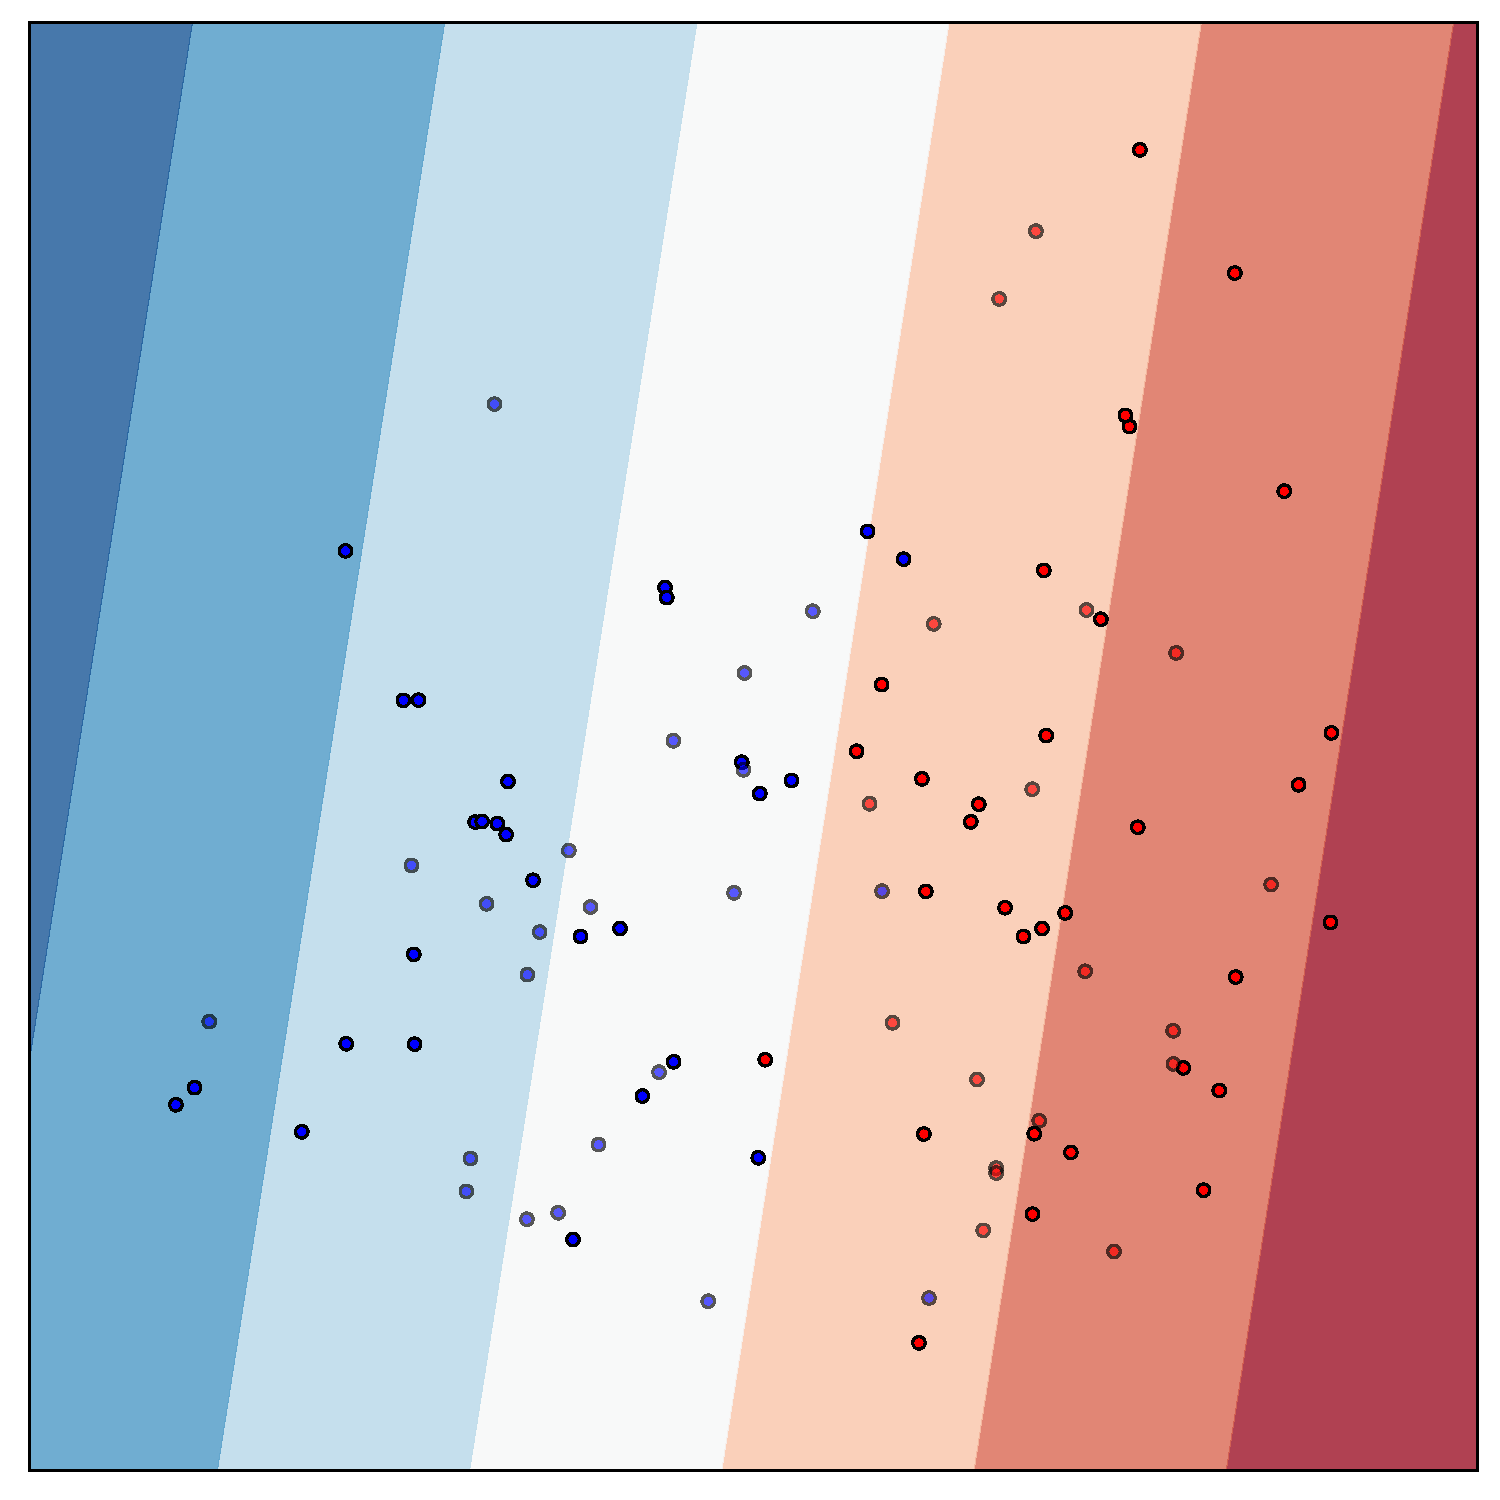
\includegraphics[width=0.75\linewidth]{figures/log_reg_classification.pdf}
        \label{fig:log_reg_classification}
    \end{subfigure}%
    \begin{subfigure}{.5\textwidth}
        \centering
        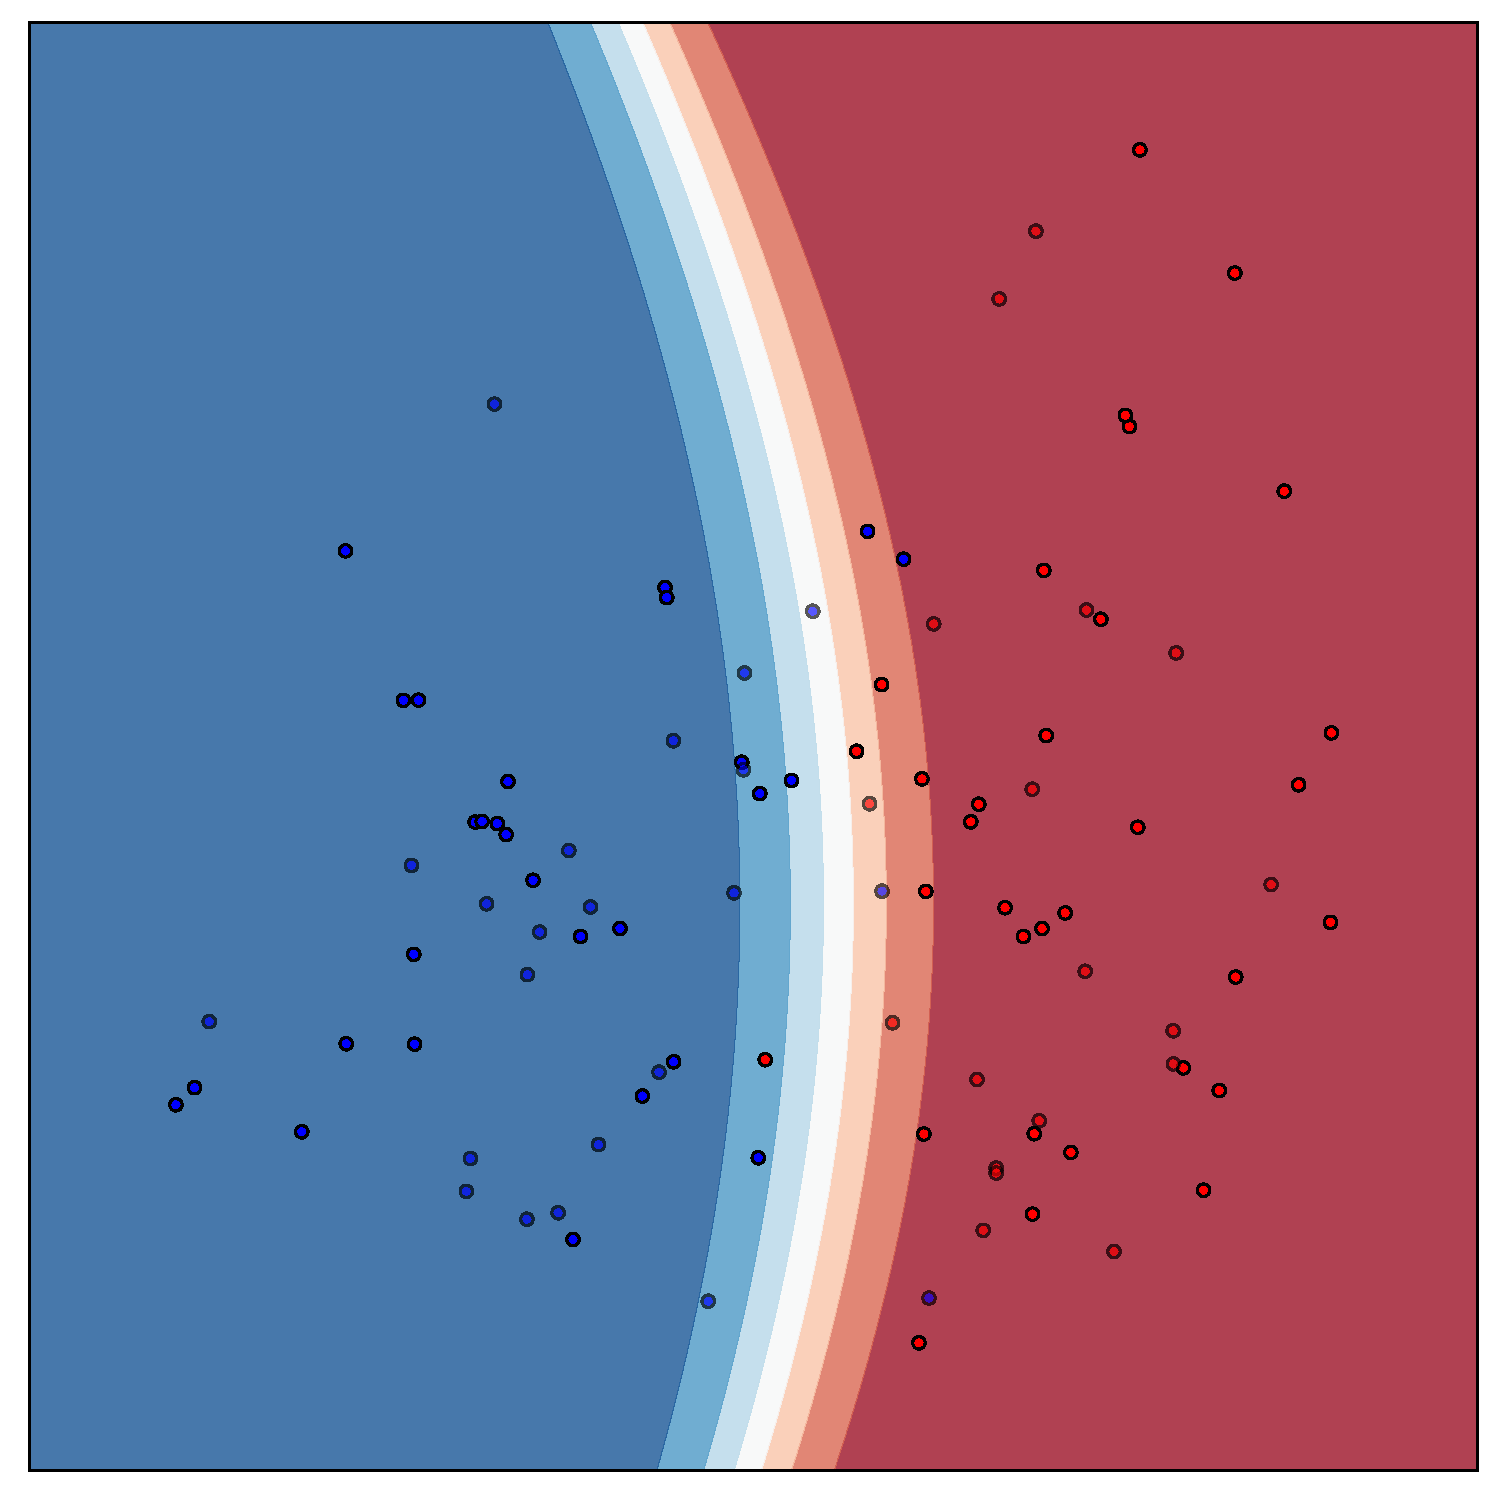
\includegraphics[width=0.75\linewidth]{figures/nb_classification.pdf}
        \label{fig:nb_classification}
    \end{subfigure}
    \caption{
        Illustration of the decision boundary for the logistic regression (left)
        and gaussian naive Bayes (right) for binary classification.
        For logistic regression, the separation is an hyperplane.
        For gaussian naive Bayes, the separation has a dependency on $x \odot x$ and can be non-linear.
        Both bernoulli and multinomial naive Bayes would have a linear separation.
    }
    \label{fig:log_reg_nb_comparison}
\end{figure}

\section{Sparse naive Bayes}\label{sec:snb}

A sparse version of naive Bayes was introduced in 2019~\cite{sparse_naive_bayes}.
They add a sparsity constraint in the Bernoulli and the multinomial optimization problems portrayed above.
It imposes the weight vector $\ww$ to have a number of non-zero entries under a certain threshold $k \in \N$.
That property is similar to the one of the Lasso presented in~\ref{subsubsec:lasso}.
But the sparsity in sparse naive Bayes (SNB) is controlled by an integer $k$ which is
the exact sparsity level desired on the weight vector,
while the Lasso relies on a continuous penalty coefficient $\lambda \in \R$.
This sparsity property makes SNB employable to perform feature selection,
by keeping only the features whose weights are non-zero.
Next sections detail the problem statement, the main results of the authors,
and some applications.

\subsection{Problem statement}\label{subsec:snb_ps}

Let $0 \leq k \leq p$ be a desired level of sparsity.
We wish to train a naive Bayes classifier whose decision boundary depends on at most $k$ features.
For any $\vv \in \R^d$ we note $\norm{\vv}_0$ the number of non-zero entries
(the cardinality) of the vector.
As shown in the previous section~\ref{subsec:nb_bound},
there exist $v \in \R$ and $\ww \in \R^p$ such that the prediction $y(\xx)$ for a new data point $\xx\in\R^p$ is
$\sign(v + \ww^\top\xx)$ for both bernoulli and multinomial naive Bayes.
Furthermore, the $j$th entry of the decision vector $\ww$ is null if and only if $\btheta^-_j = \btheta^+_j$,
where $\btheta^-$ and $\btheta^+$ are the parameters of the loss functions $\lglh_b$ and $\lglh_m$
in~\ref{eq:bernoulli_snb_ll} and~\ref{eq:multinomial_snb_ll} respectively.
Naturally, imposing the constraint $\norm{\btheta^+ - \btheta^-}_0 \leq k$ in the optimization problems
will yield a weight vector $\ww$ with the desired sparsity.
The optimization problems for Bernoulli and multinomial SNB
(shortened BSNB and MSNB respectively) can be phrased as follows:
\begin{equation}\label{eq:bsnb}\tag{BSNB}
    \begin{aligned}
        & \underset{\btheta^+,\, \btheta^-}{\text{maximize}}
        & & \lglh_\text{b}\left( \btheta^+,\, \btheta^- \right)
            \begin{split}
                &&&= \ff_+^\top\log\btheta^+ + (n_+\1 - \ff_+)^\top\log\left( \1 - \btheta^+ \right)\\
                &&&\qquad+ \ff_-^\top\log\btheta^- + (n_-\1 - \ff_-)^\top\log\left( \1 - \btheta^- \right)
            \end{split}\\
        & \text{subject to}
        & & \norm{\btheta^+ - \btheta^-}_0 \leq k.
    \end{aligned}
\end{equation}
\begin{equation}\label{eq:msnb}\tag{MSNB}
    \begin{aligned}
        & \underset{\btheta^+,\, \btheta^-}{\text{maximize}}
        & & \lglh_\text{m}\left( \btheta^+,\, \btheta^- \right) = \ff_+^\top\log\btheta^+ + \ff_-^\top\log\btheta^-\\
        & \text{subject to}
        & & \norm{\btheta^+ - \btheta^-}_0 \leq k\\
        & \text{ and }
        & & \1^\top\btheta^+ = \1^\top\btheta^- = 1.
    \end{aligned}
\end{equation}

\subsection{Main results and resolution}\label{subsec:snb_th}

Surprisingly and despite the combinatorial constraints,
these optimizations problems can be (approximately) solved very efficiently,
with an additional minor cost compared to vanilla naive Bayes.

Especially for the Bernoulli case,
an optimal solution can be computed in closed-form as shown in Theorem~\ref{th:bsnb}.
\begin{theorem}\label{th:bsnb}
    Suppose that $X \in \left\{ 0, 1 \right\}^{n \times p}$ is modeled by the Bernoulli distribution.
    Then, the exact solution to the problem~\ref{eq:bsnb} can be computed.
    First, define $\mt$ and $\uu$ as follows
    \begin{align*}
        \mt &= (\ff^+ + \ff^-) \odot \log\left( \frac{\ff^+ + \ff^-}{n} \right)
                + (n\1 - \ff^+ - \ff^-) \odot \log\left( \1 - \frac{\ff^+ + \ff^-}{n} \right)\\
        \begin{split}
                \uu &= \ff^+ \odot \log \frac{\ff^+}{n^+} + (n^+\1 - \ff^+) \odot \log (\1 - \frac{\ff^+}{n^+})\\
                &\qquad + \ff^- \odot \log \frac{\ff^-}{n^-} + (n^-\1 - \ff^-) \odot \log (\1 - \frac{\ff^-}{n^-})
        \end{split}
    \end{align*}
    Let $\cI$ be the set of $p - k$ smallest elements of $\uu - \mt$, and let
    \begin{equation*}
        {\theta^+_\star}_j = {\theta^-_\star}_j = \frac{1}{n}(f_j^+ + f_j^-)
        \;\forall j \in \cI
        ,\qquad
        {\theta^\pm_\star}_j = \frac{f^\pm_j}{n^\pm}
        \;\forall j \notin \cI
    \end{equation*}
\end{theorem}
Forming the vectors $\ff^-$ and $\ff^+$ is very quick
and takes asymptotically $\cO\left( n \cdot p \right)$ summations.
Then, constructing $\mt$ and $\uu$ can be done in $\cO\left( p \right)$ calculations.
Finding the $k$ largest elements of $\uu - \mt$ takes $\cO\left( p \cdot \log k \right)$ steps.
Finally, constituting $\btheta_\pm^\star$ requires $\cO\left( p \right)$ operations.
In total, the maximizer can be found in $\cO\left( n \cdot p + p \cdot \log k \right)$ steps,
which is very close to the cost $\cO\left( n \cdot p \right)$ of naive Bayes.

In the multinomial case, there is no closed-form solution, but a near-optimal one can be obtained as
stated in Theorem~\ref{th:msnb}.
\begin{theorem}\label{th:msnb}
    Suppose that $X \in \R_+^{n \times p}$ is modeled by the multinomial distribution.
    Then the dual of~\ref{eq:msnb} can be solved very efficiently and a good solution to the primal can be recovered.
    Define $\phi_k : \alpha \mapsto s_k(\hh(\alpha)) + C$ where $C$ is some constant,
    $s_k$ the sum of the k largest values of a vector, and
    \begin{equation*}
        \begin{split}
            \hh(\alpha) &= \ff_+ \odot \log \ff_+ + \ff_- \odot \log \ff_-
                    - (\ff_+ + \ff_-) \odot \log (\ff_+ + \ff_-)\\
                &\qquad - \ff_+ \log \alpha - \ff_- \log (1 - \alpha)
        \end{split}
    \end{equation*}
    $\phi_k$ is the dual of~\ref{eq:msnb} and can be minimized very quickly (with bisection for example)
    as it is a one-dimensional convex convex function.
    Let $\alpha^\star$ be its minimizer, $\cI$ the set of the $p - k$ smallest entries of
    $\hh(\alpha^\star)$, and $B_\pm = \sum_{j \notin \cI} f_i^\pm$.
    A primal point can be reconstructed as follows:
    \begin{equation*}
        {\theta^+_\star}_j = {\theta^-_\star}_j = \frac{f_j^+ + f_j^-}{\1^\top(\ff^+ + \ff^-)}
        \;\forall j \in \cI
        ,\qquad
        {\theta^\pm_\star}_j = \frac{B_+ + B_-}{B_\pm}\frac{f^\pm_j}{\1^\top(\ff^+ + \ff^-)}
        \;\forall j \notin \cI
    \end{equation*}
    Furthermore, it holds that $\psi(k - 4) \leq \phi(k) \leq \psi(k) \leq \phi(k + 4)$,
    implying that the duality gap is small if $\psi(k) - \psi(k - 4)$ is small.
\end{theorem}
Experimentally, the duality gap quickly converges to $0$ as $k$ increases,
and the reconstructed primal point is near-optimal.
The time complexity is once again $\cO(n \cdot p + p \cdot \log k)$,
which is a minor additional cost compared to plain naive Bayes.

The authors experiment SNB on several text datasets,
including AMZN, IMDB, TWTR, MPQA and SST2.
They compare it with more costly methods like the Lasso, $\ell_1$-penalized logistic regression and SVMs.
They obtain competitive test accuracies, while training their models several order of magnitude faster.

\section{Applications}\label{sec:nb_app}

The apparent low complexity of sparse naive Bayes compared to $\ell_1$-penalized methods such as
Lasso, logistic regression or SVMs makes is appealing for very large scale datasets.
We mention here a few applications to which we will come back later\footnote{
    An implementation of sparse naive Bayes can be found~\href{https://github.com/aspremon/NaiveFeatureSelection}{here}.
}.

\subsection{Criteo dataset}\label{subsec:snb_criteo}

As part of a Kaggle competition \emph{Display Advertising Challenge}\footnote{
    The Kaggle competition can be found at
    \href{https://www.kaggle.com/c/criteo-display-ad-challenge}{this address}.
}
in mid-2014, CriteoLabs shared log data collected over one week\footnote{
    The competition's dataset can be downloaded at
    \href{https://labs.criteo.com/2014/02/download-kaggle-display-advertising-challenge-dataset/}{this address}.
}
whose features were undisclosed for confidentiality purposes.
Main characteristics of this dataset can be found in Table~\ref{tab:criteo_dataset}.
\begin{table}[!htb]
    \centering
    \setlength{\tabcolsep}{2pt}
    {\small
    \begin{tabular}{|c|c|c|c|c|}\hline
    \textbf{Samples} & \textbf{Total features} & \textbf{Numerical features} & \textbf{Categorical features} & \textbf{Features after encoding}\\ \hline
    $45\,840\,617$ & $39$  & $13$ & $26$ & $33\,762\,590$ \\ \hline
    \end{tabular}
    }%
    \caption[short]{
        Criteo dataset characteristics.
        Even though the number of features is small,
        most categorical features have millions of categories.
        It makes the training of predicting models particularly challenging as it requires several
        dozens of GB of memory.
    }
    \label{tab:criteo_dataset}
\end{table}
It consists in $\approx 45$ millions of display ads with 39 features,
and a boolean label describing whether or not the ad was clicked by a customer.
Among these 39 features, 26 are categorical and a classical one-hot encoding would end up in millions of features.
This makes the Criteo dataset challenging, as it doesn't fit in the random-access memory after encoding,
and potentially not in the mass storage of a standard computer either.
Even on a small subset of the features, say 10\%,
selecting important features using Lasso or $\ell_1$-penalized logistic regression isn't realistic.
One-hot encoding isn't adapted to that situation.
Another approach would be to one-hot encode for each categorical feature only the most frequent categories,
and put the rest in a category \textit{other}.
The winners of the Kaggle competition used the hashing trick.
It consists in choosing an encoding space size $m$,
for example $m = 2^{20}$,
and defining some hash function $h \colon \text{Categories} \to \left\{ 0, \dots, m - 1 \right\}$.
This approach has several notable advantages.
First, the final encoded feature space $m$ can be adapted depending on the needs and on the computing power.
It may be used in an online fashion without a first pass
(that would be required for one-hot encoding in order to figure out all the existing categories).
Lastly, it naturally handles new labels in the test set that were unseen in the train set
(which would typically need a special \textit{other} category in the one-hot encoding setting).
Collisions between categories are likely to happen,
and even collisions between categories from different features.

We present here in Figure~\ref{fig:criteo_hash_elbow}.
$m = 2^{24} = 16777216$
All the computations are done on a standard workstation (16GB, Intel Core i7 3.60GHz $\times$ 8).
Sparse naive Bayes requires data averages to run,
i.e.\ the sums of the negative and of the positive points.
This part is time consuming but once these sums are computed they can be reused for any sparsity level $k$.
Using a light hash function and PyPy, they were obtained in around 20 minutes.
Only roughly half of the $2^{24}$ hash features were hit by the hash function.
Then, SNB optimum are computed for 1200 log-spaced points using a Python and NumPy implementation of SNB in 1 hour.
In this situation, what makes SNB particularly appealing is the fact that at no moment we need to load the full dataset
in memory.
We are only computing data averages whose shape are much smaller than the full matrix.
Note also that most tasks could even be distributed to speed up the computations.
\begin{figure}
    \centering
    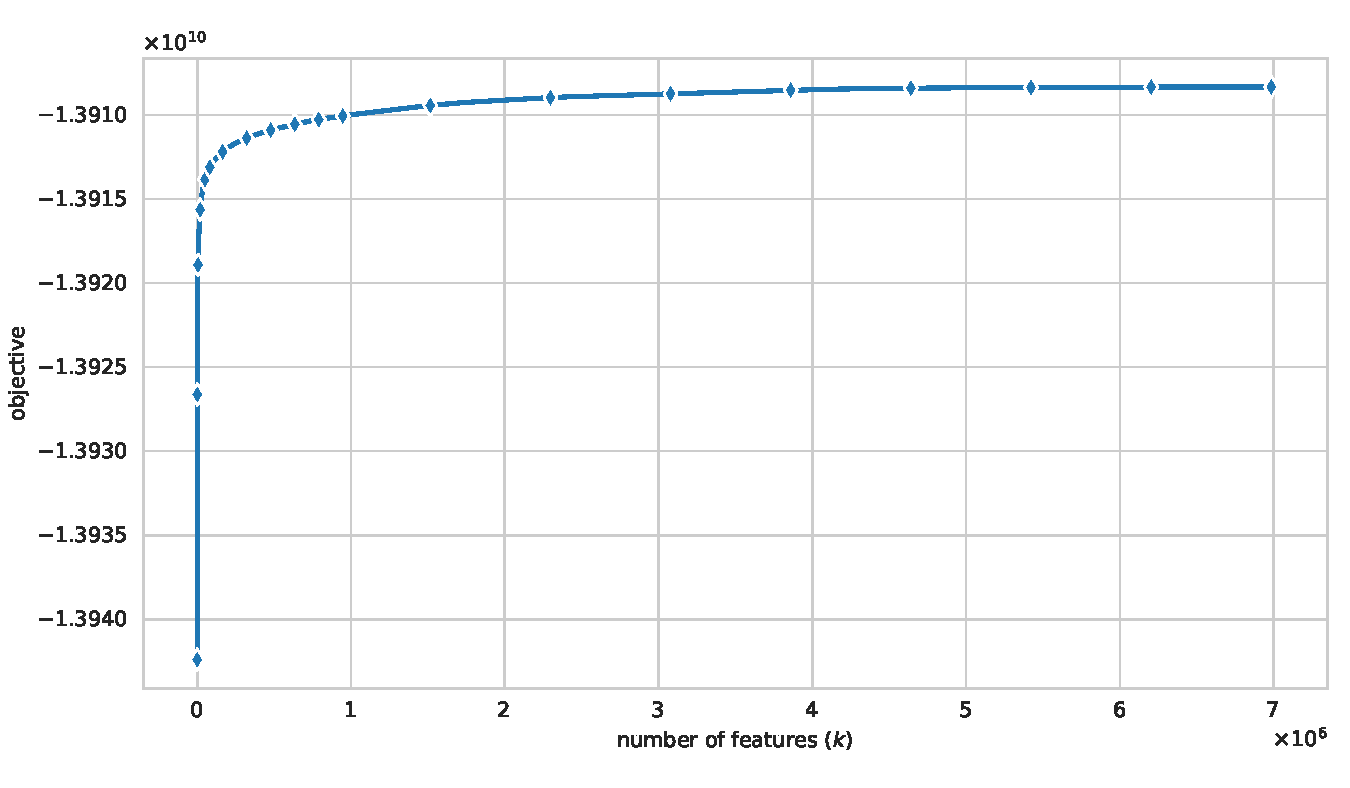
\includegraphics[width=0.75\linewidth, height=0.4\linewidth]{figures/criteo_hash_elbow.pdf}
    \caption{
        Optimal value of the~\ref{eq:msnb} optimization problem on the Criteo dataset
        as a function of the sparsity parameter $k$.
        Only 1--2 millions of the features explain most of the target vector (elbow heuristic).
    }
    \label{fig:criteo_hash_elbow}
\end{figure}

\subsection{Genetic and fMRI data}\label{subsec:snb_genetic_fmri}



\bigbreak
Finally, sparse naive Bayes appear as an attractive alternative to the Lasso for the statistics computation
in the knockoff procedure~\ref{sec:ksc}.
